\section{Iterative PlasBin-flow binning method}

In the following, a fragment can refer to both a pangenome fragment or a contig.
As an abuse of notation, we use in the whole section the set \Fragments{} to denote either the pan-assembly fragment set or the contig set.

The here presented Iterative PlasBin-flow binning method is an adaptation of the original PlasBin-flow method~\cite{manePlasBinflowFlowbasedMILP2023}.

The binning method consists in iteratively find the best bin by solving a flow-based combinatorial optimization problem on a network graph (defined in \Cref{sec:pbf_iterbin:network}).
Once a bin is found, we extract it from the network and continue the search until some criterion are not met.
For a given bin, each fragment is associated with a use of its coverage.
Extracting the bin from the network graph means decreasing the fragment coverages in the graph.
When the coverage a fragment in the network falls to zero, the fragment and its arcs are removed from graph.
\Cref{algo:pbf_iterbin} details the iterative binning process.

\begin{tcbalgo}{Iterative PlasBin-flow binning}{pbf_iterbin}
  \begin{algorithmic}[1]
    \Require{%
      A network graph \(N\) as defined in \Cref{sec:pbf_iterbin:network}.
    }
    \Ensure{%
      Extract bins from the network graph.
    }
    \Function{extract\_bins}{\( N \)}
    \While{There are seeds in \(N\) and the previous model was feasible}
    \State{} \( find\_result \gets \Call{find\_best\_bin}{ N } \)
    \If{\( find\_result.\Call{feasibility\_message}{  } \) is a feasible message}
    \State{} Output \( find\_result.\Call{bin}{ } \)
    \State{} Extract the bin from the network graph \(N\) by updating the coverages.
    \EndIf{}
    \EndWhile{}
    \EndFunction{}
  \end{algorithmic}
\end{tcbalgo}

We propose three Mixed Integer Linear Programming (MILP) approaches to find the best bin (\( \Call{find\_best\_bin}{} \) subfunction, \Cref{sec:pbf_iterbin:decomp,sec:pbf_iterbin:binlab,sec:pbf_iterbin:once})
Each of them tries to answer to the PlasBin-flow discussion.

\begin{newfeatbox}
  Comparing to PlasBin-flow, we directly model the flow connectivity in the MILP models.
\end{newfeatbox}

The MILP models share subsets of variables and constraints we detail in \Cref{sec:pbf_iterbin:milp}.

%
% Common parts among the approaches
%
\subsection{The network graph}\label{sec:pbf_iterbin:network}

All the MILP flow-based approaches are built on the top of a flow network:

\begin{itemize}
  \item We add two vertices, \source{} and \sink{}, that are respectively the source and the sink vertices.
  \item The set \(\VSeeds{}\) contains the vertices associated with the seed contigs in \ContigSeeds{}.
    The source goes into each vertex in \(\VSeeds{}\), and each vertex in \(V_{\Contigs{}}\) goes into the sink.
\end{itemize}

\begin{notebox}
  We discuss in \zcref[S]{sec:pbf_iterbin:conclusions} the connection of the source to only the seeds.
\end{notebox}

\begin{definition}{Network graph}{pbf_iterbin:network_graph}
  Let \(N = (V, A, \source{}, \sink{}, \cov{\Contigs{}}, \gcscore{\Contigs{}}{K}, \plm{\Contigs{}})\) be the network graph, where:

  \begin{itemize}
    \item \( V = V_\Contigs{} \cup \Set*{\source{}, \sink{}} \) is the set of vertices with the source \(\source{}\) and the sink \(\sink{}\);
    \item \( A = A_\Links{} \cup \Set{(\source, v) \given v \in \VSeeds{}} \cup \Set{(v, \sink) \given v \in V} \) is the set of link-arcs augmented with the source-arcs and the sink-arcs;
    \item \( \cov{\Contigs{}} \colon \Contigs{} \to \Reals{}_{> 0} \) is the coverage function;
    \item \( \gcscore{\Contigs{}}{K} \colon \Contigs{} \times K \to [-1, 1] \) is the GC score function;
    \item \( \plm{\Contigs{}} \colon \Contigs{} \to [-1, 1] \) is the plasmidness function.
  \end{itemize}
\end{definition}


\subsection{Common Mixed Integer Linear Programming (MILP) objects}\label{sec:pbf_iterbin:milp}

\Cref{tab:pbf_iterbin:milp:variables} lists all the variables used in the MILP models.

\begin{table}
  \centering
  \tablecaptionof{MILP variable set}{%
    Each of the following variables participates in at least one of the MILP model.
    Some of them participate in all the model, others are necessary for only one model.
    For the ease of read, we categorize the variables in three categories.
    Each section describing a model precise which variables are participating for each category.
  }\label{tab:pbf_iterbin:milp:variables}

  \begin{longtable}{@{}llp{0.5\textwidth}@{}}
    \toprule
    \tabhtxt{Variable} & \tabhtxt{Application set} & \tabhtxt{Meaning} \\
    \midrule
    %
    \multicolumn{3}{@{}l@{}}{\tabhtxt{Decision variables}} \\
    \addlinespace
    \(x_v \in \Reals_{\geq 0}\) & \(\forall v \in V \setminus \Set*{s, t}\) & Denoting whether the vertex \(v\) is active or not. \\
    \addlinespace
    \(y_a \in \Set{0, 1}\) & \(\forall a \in A_\Links{}\) & Denoting whether the link-arc \(a\) is active or not. \\
    \addlinespace
    \(\frag{i} \in [0, 1] \) & \(\forall i \in \Fragments{}\) & Denoting whether fragment \(i\) is active or not. With the constraints it acts as a binary. \\
    \addlinespace
    \(GC_b \in \Set{0, 1}\) & \(\forall b \in K\) & Denoting whether the plasmid GC content is in the GC content interval \(b\) or not. \\
    \addlinespace
    \(\fraggc{i}{b} \in \Reals_{\geq 0}\) & \(\forall (i, b) \in \Fragments{} \times K\) & Denoting whether the fragment \(i\) is active and the plasmid GC content is in the interval \(b\) or not. With the constraints it acts as a binary. \\
    %
    \addlinespace
    \multicolumn{3}{@{}l@{}}{\tabhtxt{Flow variables}} \\
    \addlinespace
    \(f_a \in \Reals_{\geq 0}\) & \(\forall a \in A_\Links{}\) & Corresponding to the flow amount passing through the link-arc \(a\). \\
    \addlinespace
    \(F \in \Reals_{\geq 0}\) & & Corresponding to the overall flow. \\
    \addlinespace
    \(F_a \in \Reals_{\geq 0}\) & \(\forall a \in A_\Links{}\) & Playing the role of an intermediary variable to force the flow on each link-arc to be equal to the total flow. \\
    \addlinespace
    \(\inflowgc{i}{b} \in \Reals_{\geq 0}\) & \(\forall (i, b) \in \Fragments{} \times K\) & Corresponding to the flow amount passing through the fragment \(i\) when the plasmid GC content is in the interval \(b\). \\
    %
    \addlinespace
    \multicolumn{3}{@{}l@{}}{\tabhtxt{Connected component variables}} \\
    \addlinespace
    \(\alpha \in \Reals{}\) & & Is the number of \emph{oriented} fragments in the solution connected graph, plus the source and the sink. With the constraints it acts as a positive integer. \\
    \addlinespace
    \(\beta_a \in \Reals_{\leq 0}\) & \(\forall a \in A_\Links{}\) & Is strictly negative if the link-arc \(a\) participates in one of the solution subgraph's exploration tree. It acts as a negative integer, where the absolute value corresponds to the depth of the subtree defined by the successor. \\
    %
    \bottomrule
  \end{longtable}
\end{table}
Here we describe and categorize the set of constraints composing the different MILP models.
In what follow, we define either a fragment, a contig or an arc to be \enquote{active} if it participates in the solution, i.e.\ the flow passes through it.

\paragraph{Decision variables relationships}

A fragment is active if, and only if at least one of its extremity vertices is active:
\begin{align}
  x_v & \leq \frag{i} & \forall v \in V \setminus \Set*{s, t}, i = vfrag(v) \cstlabel{pbf_iterbin:milp:cst:dvar:active_extremity_implies_active_fragment} \\ % chktex 25
  \frag{i} & \leq x_u + x_v & \forall i \in \Fragments{}, \{u, v\} \in \EFrags{} \cstlabel{pbf_iterbin:milp:cst:dvar:active_fragment_implies_active_extremity} % chktex 25
\end{align}

The fragments involved in an active link-arc must also be active:
\begin{equation}
  y_{uv} \leq
  \begin{cases}
    x_v & \text{if \(u = s\)} \\
    x_u & \text{if \(v = t\)} \\
    \min\Set{x_u, x_v} & \text{otherwise}
  \end{cases} \quad \forall (u, v) \in A_\Links{} %
  \cstlabel{pbf_iterbin:milp:cst:dvar:active_link_arc_active_fragments} % chktex 25
\end{equation}

An active vertex implies at least one active link-arc incoming to it:
\begin{questionbox}
  Are these constraints necessary?
\end{questionbox}
\begin{equation}
  x_v \leq \sum_{(u, v) \in A_\Links{}} y_{u v} \quad \forall v \in V \setminus \Set{s, t} \cstlabel{pbf_iterbin:milp:cst:dvar:active_vertex_active_incoming_arcs} % chktex 25
\end{equation}

\paragraph{Flow constraints}

The flow through a link-arc \(a \in A_\Links{}\) is non-zero if \(a\) is active and cannot exceed its capacity:
\begin{align}
  f_{uv} \leq
  \begin{cases}
    \cov{j} y_{uv} & \text{if \(u = s\)} \\
    \cov{i} y_{uv} & \text{if \(v = t\)} \\
    \min\Set*{\cov{i}, \cov{j}} y_{uv} & \text{otherwise}
  \end{cases} &
  \begin{split}
    \forall (u, v) \in A_\Links{} \\
    i = vfrag(u) \\
    j = vfrag(v)
  \end{split} \cstlabel{pbf_iterbin:milp:cst:flow:arc_flow_at_most_coverage} % chktex 25
\end{align}

The cumulative flow through a fragment \(i \in \Fragments{}\) cannot exceed its read coverage:
\begin{equation}
  inflow(i) \leq \cov{i} \quad \forall i \in \Fragments{} \cstlabel{pbf_iterbin:milp:cst:flow:inflow_at_most_coverage} % chktex 25
\end{equation}
Where \(\displaystyle inflow(i) = \sum_{(u, i_t) \in A_\Links{}} f_{ui_t} + \sum_{(u, i_h) \in A_\Links{}} f_{ui_h}\) where \(i_t\) and \(i_h\) respectively stand for the tail and the head vertices of fragment \(i\).

The cumulative flow into a fragment \(i\) should be equal to the cumulative flow out of it. Same for the reverse \(i^-\):
\begin{align}
  \sum_{(u, i_t) \in A_\Links{}} f_{u i_t} & = \sum_{(i_h, w) \in A_\Links{}} f_{i_h w} & \forall i \in \Fragments{} \cstlabel{pbf_iterbin:milp:cst:flow:inflow_equals_outflow_forward} \\ % chktex 25
  \sum_{(u, i_h) \in A_\Links{}} f_{u i_h} & = \sum_{(i_t, w) \in A_\Links{}} f_{i_t w} & \forall i \in \Fragments{} \cstlabel{pbf_iterbin:milp:cst:flow:inflow_equals_outflow_reverse} % chktex 25
\end{align}

The total flow value \(F\) equals to the flow out of \(s\) and into \(t\):
\begin{align}
  F & = \sum_{(s, v) \in A_\Links{}} f_{sv} \cstlabel{pbf_iterbin:milp:cst:flow:total_flow_source} \\ % chktex 25
  F & = \sum_{(v, t) \in A_\Links{}} f_{vt} \cstlabel{pbf_iterbin:milp:cst:flow:total_flow_sink} % chktex 25
\end{align}

The total flow is strictly positive:
\begin{equation}
  F \geq \epsilon_F \quad \epsilon_F > 0 \cstlabel{pbf_iterbin:milp:cst:flow:total_flow_strictly_positive} % chktex 25
\end{equation}

An active link-arc has a flow at least \(F\).
\begin{align}
  F_a & \geq F - (1 - y_a) \max_{i \in \SeedFrags{}}\Set{\cov{i}} & \forall a \in A_\Links{} \cstlabel{pbf_iterbin:milp:cst:flow:arc_flow_at_least_total_flow_1} \\ % chktex 25
  F_a & \leq F & \forall a \in A_\Links{} \cstlabel{pbf_iterbin:milp:cst:flow:arc_flow_at_least_total_flow_2} \\ % chktex 25
  F_a & \leq f_a & \forall a \in A_\Links{} \cstlabel{pbf_iterbin:milp:cst:flow:arc_flow_at_least_total_flow_3} % chktex 25
\end{align}
\begin{infobox}
  These constraints do not force the arc flows to be a multiple of \(F\), see~\Cref{proposition:inflow_is_not_multiple_of_total_flow}.
\end{infobox}
\begin{missingproofbox}
  The above constraints minimize the number of out link-arcs for each fragment.
\end{missingproofbox}
\begin{questionbox}
  What is the meaning for a fragment to have a cumulative flow that is not a multiple of \(F\)?
  By keeping the flow real, can we smartly force the cumulative flow to be a multiple of \(F\)?
\end{questionbox}

\paragraph{Connected component constraints}

Exactly one link-arc outs of \(s\) is part of the solution (necessary to ensure the solution induced subgraph has only one connected component):
\begin{equation}
  \sum_{(s, v) \in A_\Links{}} y_{sv} = 1 \cstlabel{pbf_iterbin:milp:cst:ccomp:one_outgoing_arc_from_source} % chktex 25
\end{equation}

A positive flow implies the two incident vertices are in the component:
\begin{equation}
  1 - y_{uv} \geq
  \begin{cases}
    1 - x_v & \text{if \(u = s\)} \\
    x_u - 1 & \text{if \(v = t\)} \\
    x_u - x_v & \text{otherwise}
  \end{cases}
  \quad \forall (u, v) \in A_\Links{}
  \cstlabel{pbf_iterbin:milp:cst:ccomp:positive_flow_incident_vertices_in_component} % chktex 25
\end{equation}
\begin{questionbox}
  potentially redundant with \Cref{pbf_iterbin:milp:cst:dvar:active_vertex_active_incoming_arcs}
\end{questionbox}

The cumulative depth of the subtree in the exploration tree from the source equals at least the number of active vertices minus 1.
\begin{align}
  \alpha + \sum_{(s, w) \in A_\Links{}} \beta_{sw} \leq 1 \cstlabel{pbf_iterbin:milp:cst:ccomp:depth_of_tree_source} % chktex 25
\end{align}

Two incident arcs in the exploration tree are distanced by one.
\begin{align}
  \sum_{(v, w) \in A_\Links{}} \beta_{vw} - \sum_{(u, v) \in A_\Links{}} \beta_{uv} \leq 1 \quad \forall v \in V \setminus \Set*{s}
  \cstlabel{pbf_iterbin:milp:cst:ccomp:depth_of_tree_incident_arcs} % chktex 25
\end{align}

An arc participates in the exploration tree implies the arc is active.
\begin{align}
  \beta_a \geq - y_a |V| \quad \forall a \in A_\Links{}
  \cstlabel{pbf_iterbin:milp:cst:ccomp:tree_arc_active} % chktex 25
\end{align}

The number of active vertices equals \(\alpha{}\) (SAT constraint):
\begin{align}
  2 + \sum_{v \in V \setminus \Set*{s, t}} x_v = \alpha
  \cstlabel{pbf_iterbin:milp:cst:ccomp:number_of_active_vertices} % chktex 25
\end{align}

\paragraph{GC constraints}
%
The following constraints define the GC content labelling of a bin.

\phantom{text}

Only one GC content interval \(b \in K\) labels the bin:
\begin{equation}
  \sum_{b \in K} GC_b = 1
  \cstlabel{pbf_iterbin:milp:cst:gc:exactly_one_gc_content_interval} % chktex 25
\end{equation}

For each fragment \(i \in \Fragments{}\), for each GC content interval \(b \in K\), \(\fraggc{i}{b} = 1\) if and only if fragment \(i\) is active and the bin is labelled by the GC content interval \(b\):
\begin{align}
  \fraggc{i}{b} & \leq x_{i_t} + x_{i_h} & \forall (i, b) \in \Fragments{} \times K \cstlabel{pbf_iterbin:milp:cst:gc:active_fragment_gc_1} \\ % chktex 25
  \fraggc{i}{b} & \leq GC_b & \forall (i, b) \in \Fragments{} \times K \cstlabel{pbf_iterbin:milp:cst:gc:active_fragment_gc_2} \\ % chktex 25
  \fraggc{i}{b} & \geq x_{i_t} + GC_b - 1 & \forall (i, b) \in \Fragments{} \times K \cstlabel{pbf_iterbin:milp:cst:gc:active_fragment_gc_3} \\ % chktex 25
  \fraggc{i}{b} & \geq x_{i_h} + GC_b - 1 & \forall (i, b) \in \Fragments{} \times K \cstlabel{pbf_iterbin:milp:cst:gc:active_fragment_gc_4} % chktex 25
\end{align}

For each fragment \(i \in \Fragments{}\), for each GC content interval \(b \in K\), \(\inflowgc{i}{b}\) is the flow into fragment \(i\) when \(b\) is the chosen GC content interval:
\begin{align}
  \inflowgc{i}{b} & \leq \cov{i} \frag{i} *  & \forall (i, b) \in \Fragments{} \times K \cstlabel{pbf_iterbin:milp:cst:gc:inflowgc_1}  \\ % chktex 25
  \inflowgc{i}{b} & \leq \cov{i} GC_b & \forall (i, b) \in \Fragments{} \times K \cstlabel{pbf_iterbin:milp:cst:gc:inflowgc_2}  \\ % chktex 25
  \inflowgc{i}{b} & \geq inflow(i)  - (2 - \frag{i} - GC_b) \cov{i} & \forall (i, b) \in \Fragments{} \times K \cstlabel{pbf_iterbin:milp:cst:gc:inflowgc_3} % chktex 25
\end{align}

\paragraph{Plasmid constraints}

The cumulative fragment length is above a given threshold:
%
\begin{equation}
  \sum_{i \in \SeedFrags{}} |i| \geq L \quad L \geq 0 \cstlabel{pbf_iterbin:milp:cst:misc:min_cumulative_fragment_length} % chktex 25 chktex 35
\end{equation}
%
Typically, we choose \(L = 1000\).

%
% Approaches
%
\subsection{Approach \texttt{decomp}}\label{sec:pbf_iterbin:decomp}

\begin{newfeatbox}
  At the opposite of PlasBin-flow, we split each objective expression into different mono-objective functions that define different optimization problems.
\end{newfeatbox}
The \texttt{decomp} approach tackles the binning of the contigs with a coarse-to-fine-grain approach in four stages (each one refering to an optimization problem):

\begin{enumerate}[label=\roman*.]
  \item Find the maximum coverage flow (\MCF{} problem, \zcref[S]{sec:pbf_iterbin:decomp:mcf})
  \item Find the maximum GC score (\MGC{} problem, \zcref[S]{sec:pbf_iterbin:decomp:mgc})
  \item Find the maximum plasmidness score (\MPS{} problem, \zcref[S]{sec:pbf_iterbin:decomp:mps})
  \item Refine the solution (\MRCF{} problem, \zcref[S]{sec:pbf_iterbin:decomp:mrcf})
\end{enumerate}

\zcref[S]{algo:pbf_iterbin:decomp} summarizes the \texttt{decomp} approach.

\begin{tcbalgo}{\texttt{decomp} approach}{pbf_iterbin:decomp}
  \begin{algorithmic}[1]
    \Require{%
      A network graph \(N\) as in \zcref[S]{definition:pbf_iterbin:network_graph}.
    }
    \Ensure{%
      Extract the best bin from the network graph.
    }
    \Function{find\_best\_bin}{\( N \)}
    \State{} Init \MCF{} and solve it
    \If{\MCF{} is unfeasible}
    \State{} \Return{}unfeasible message
    \EndIf{}
    \State{} Init \MGC{} from \MCF{} result and solve it
    \If{\MGC{} is unfeasible}
    \State{} \Return{}unfeasible message
    \EndIf{}
    \State{} Init \MPS{} from \MGC{} result and solve it
    \If{\MPS{} is unfeasible}
    \State{} \Return{}unfeasible message
    \EndIf{}
    \State{} Init \MRCF{} from \MPS{} result and solve it
    \If{\MRCF{} is unfeasible}
    \State{} \Return{}unfeasible message
    \EndIf{}
    \State{} \Return{}\MRCF{} bin result (defined by the MILP solution variables induced subgraph)
    \EndFunction{}
  \end{algorithmic}
\end{tcbalgo}

Between each step, we fix the objective value of the previous step.
A final step refines the solution found in the \MPS{} step (\zcref[S]{sec:pbf_iterbin:decomp:mrcf}).

\subsubsection{The Maximum Coverage-likelihood Flow problem \MCF{}}\label{sec:pbf_iterbin:decomp:mcf}

The first binning stage consists in finding a flow maximizing the use of contig coverage.
We refer to this subproblem as the \enquote{Maximum Coverage-likelihood Flow} problem (\MCF{}).
As a coarse-grain strategy, it consists in finding a connected component explaining the coverages, large enough to contain all the contigs of the in-building solution bin.
Indeed, passing through a loop or a cycle will not change the flow value. Only maximizing the flow can lead to use a minimum of contigs.
To overcome this bias, we score the use of the contig coverages and maximize their total.
Below we describe the MILP model.

\begin{table}[h!]
  \centering
  \tablecaption{\MCF{} MILP constraints}{}\label{tab:decomp:mcf:cst}
  \begin{tabular}{@{}ll@{}}
    \toprule
    \tabhtxt{Category} & \tabhtxt{Constraints} \\
    \midrule
    Decision & \zcref[S]{%
      pbf_iterbin:milp:cst:dvar:active_vertex_implies_active_contig,%
      pbf_iterbin:milp:cst:dvar:active_contig_implies_active_vertex,%
      pbf_iterbin:milp:cst:dvar:active_arc_active_vertices,%
      pbf_iterbin:milp:cst:dvar:active_vertex_active_incoming_arcs%
    } \\
    Flow & \zcref[S]{%
      pbf_iterbin:milp:cst:flow:arc_flow_at_most_coverage,%
      pbf_iterbin:milp:cst:flow:inflow_at_most_coverage,%
      pbf_iterbin:milp:cst:flow:flow_conservation,%
      pbf_iterbin:milp:cst:flow:total_flow_strictly_positive,%
      pbf_iterbin:milp:cst:flow:total_flow_source,%
      pbf_iterbin:milp:cst:flow:total_flow_sink,%
      pbf_iterbin:milp:cst:flow:arc_flow_at_least_total_flow_1,%
      pbf_iterbin:milp:cst:flow:arc_flow_at_least_total_flow_2,%
      pbf_iterbin:milp:cst:flow:arc_flow_at_least_total_flow_3%
    } \\
    Connected component & \zcref[S]{%
      pbf_iterbin:milp:cst:ccomp:one_outgoing_arc_from_source,%
      pbf_iterbin:milp:cst:ccomp:positive_flow_incident_vertices_in_component,%
      pbf_iterbin:milp:cst:ccomp:depth_of_tree_source,%
      pbf_iterbin:milp:cst:ccomp:depth_of_tree_incident_arcs,%
      pbf_iterbin:milp:cst:ccomp:tree_arc_active,%
      pbf_iterbin:milp:cst:ccomp:number_of_active_vertices%
    } \\
    GC & --- \\
    Miscellaneous & \zcref[S]{%
      pbf_iterbin:milp:cst:misc:min_cumulative_contig_length%
    } \\
    \bottomrule
  \end{tabular}
\end{table}

\begin{definition}{\MCF{} MILP objective function}{pbf_iterbin:decomp:mcf:obj}
  \begin{newfeatbox}
    Here we maximize the coverage scores, not only the coverage flow.
  \end{newfeatbox}
  %
  The objective function aims to maximize the total coverage scores:
  \begin{Objective}
    \begin{equation}
      \max ~ CoverageScore
      \label{pbf_iterbin:decomp:mcf:obj:max_coverage_score} % chktex 25 % chktex 35
    \end{equation}
  \end{Objective}
  where
  \begin{align*}
    CoverageScore & = \sum_{i \in \Contigs{}} \fzeta{i} \parenth*{ inflow(i) - (\cov{i}\contig{i} - inflow(i)) } \\
    \fzeta{i} & = \frac{ |i| }{ \max_{j \in \Contigs{}} |j| }
  \end{align*}

  \begin{notebox}
    Before we had \(
      \displaystyle CoverageScore = %
      \sum_{i \in \Contigs{}} \parenth*{2 \frac{inflow(i)}{\cov{i}} - 1}
    \)
  \end{notebox}

  \begin{ideabox}
    You can get inspired from the future multi-flow ideas and define the coverage score to be:
    \[
      CoverageScore = \sum_{
        \substack{
          i \in \Contigs{} \\
          \plm{i} > 0
        }
      } |i| \parenth*{ inflow(i) - \cov{i} }
    \]
    where we focus on the use of positive plasmidness contigs, and try to minimize the penalty of not using their coverage.
    Multipliying by the contig length keep the things robust against the fragmentation of the sequences (good property for the assembly-consensus fragments).
  \end{ideabox}
\end{definition}
\subsubsection{The Maximum GC Score problem \MGC{}}\label{sec:pbf_iterbin:decomp:mgc}

The second binning stage consists in finding a flow maximizing the GC scores, by fixing the coverage score flow.
We refer to this subproblem as the \enquote{Maximum GC Score} problem (\MGC{}).
In the following we describe the MILP model.

\begin{table}[h!]
  \centering
  \tablecaption{\MGC{} MILP constraints}{}\label{tab:decomp:mgc:cst}
  \begin{tabular}{@{}ll@{}}
    \toprule
    \tabhtxt{Category} & \tabhtxt{Constraints} \\
    \midrule
    \multicolumn{2}{@{}l@{}}{Constraints in \zcref[S]{tab:decomp:mcf:cst}} \\
    \addlinespace
    GC & \zcref[S]{%
      pbf_iterbin:milp:cst:gc:exactly_one_gc_content_interval,%
      pbf_iterbin:milp:cst:gc:active_contig_gc_1,%
      pbf_iterbin:milp:cst:gc:active_contig_gc_2,%
      pbf_iterbin:milp:cst:gc:active_contig_gc_3,%
      pbf_iterbin:milp:cst:gc:active_contig_gc_4%
    } \\
    \MGC{} dedicated & \zcref[S]{pbf_iterbin:decomp:mgc:cst:fix_mcf_obj} \\
    \bottomrule
  \end{tabular}
\end{table}

In addition to the constraints in \zcref[S]{tab:decomp:mgc:cst}, we constraint the coverage score to be near to the optimal coverage score \(\Phi{}\) previously found in \MCF{}:
\begin{Constraint}
  \begin{equation}
    \Phi - (1 - \gamma_1) | \Phi | \leq CoverageScore \quad \gamma_1 \in (0.5, 1] % chktex 9
    \label{pbf_iterbin:decomp:mgc:cst:fix_mcf_obj} % chktex 25
  \end{equation}
\end{Constraint}

\begin{definition}{\MGC{} MILP objective function}{pbf_iterbin:decomp:mgc:obj}
  The objective function aims to maximize the GC score:
  \begin{Objective}
    \begin{equation}
      \max ~ GCScore
      \label{pbf_iterbin:decomp:mgc:obj:max_gc_probability_score} % chktex 25 % chktex 35
    \end{equation}
  \end{Objective}
  where \(
    \displaystyle GCScore = \sum_{\substack{
        i \in \Fragments{} \\
        b \in K
    }} \gcscore{i}{b} \fraggc{i}{b}%
  \).

  \begin{notebox}
    In the opposite of the other \texttt{decomp} models, in \MGC{} the GC score does not depend on the fragment coefficient \fzeta{i}.
  \end{notebox}
\end{definition}
\subsubsection{The Maximum Plasmidness Score problem \MPS{}}\label{sec:pbf_iterbin:decomp:mps}

The third binning stage consists in finding a flow maximizing the plasmidness scores, by fixing both the coverage flow and the GC score.
We refer to this subproblem as the \enquote{Maximum Plasmidness Score} problem (\MPS{}).
In the following we describe the MILP model.

\begin{table}[h!]
  \centering
  \tablecaption{\MPS{} MILP constraints}{}\label{tab:decomp:mps:cst}
  \begin{tabular}{@{}ll@{}}
    \toprule
    \tabhtxt{Category} & \tabhtxt{Constraints} \\
    \midrule
    \multicolumn{2}{@{}l@{}}{Constraints in \zcref[S]{tab:decomp:mgc:cst}} \\
    \addlinespace
    \MPS{} dedicated & \zcref[S]{pbf_iterbin:decomp:mps:cst:fix_mgc_obj} \\
    \bottomrule
  \end{tabular}
\end{table}

The total GC score value must be near to the total GC score best value \(\Psi{}\) previously found in \MGC{}:
\begin{Constraint}
  \begin{equation}
    \gamma_2 \Psi \leq GCScore \quad \gamma_2 \in (0.5, 1] % chktex 9
    \label{pbf_iterbin:decomp:mps:cst:fix_mgc_obj} % chktex 25
  \end{equation}
\end{Constraint}

\begin{definition}{\MPS{} MILP objective function}{pbf_iterbin:decomp:mps:obj}
  \begin{newfeatbox}
    While in the original PlasBin-flow method the plasmidness is positive, here the it either acts as a bonus or a penalty (\( \plm{i} \in [-1, 1] \)).
  \end{newfeatbox}
  %
  The objective function aims to maximize the plasmidness scores:
  \begin{Objective}
    \begin{equation}
      \max ~ PlasmidnessScore
      \label{pbf_iterbin:decomp:mps:obj:max_plasmidness_score} % chktex 25 % chktex 35
    \end{equation}
  \end{Objective}
  where \(\displaystyle PlasmidnessScore = \sum_{i \in \Fragments{}} \fzeta{i} \plm{i} \frag{i}\).
\end{definition}

\subsubsection{The Maximum Refined Coverage-likelihood Flow problem \MRCF{}}\label{sec:pbf_iterbin:decomp:mrcf}

The solution set \(S_\MPS{}\) for \MPS{} contains solutions with the same value of \(PlasmidnessScore\) and different values for \(CoverageFlow\) and \(GCScore\) because of \Cref{pbf_iterbin:decomp:mgc:cst:fix_mcf_obj,pbf_iterbin:decomp:mps:cst:fix_mgc_obj}.
The final refinement stage consists in fixing the value of \(PlasmidnessScore\) and finding the subset of \(S_\MPS{}\) maximizing first \(CoverageFlow\) and then \(GCScore\).
It results in a last MILP formulation \(\MRCF{}\):

\begin{table}[h!]
  \centering
  \tablecaption{\MRCF{} MILP constraints}{}\label{tab:decomp:mrcf:cst}
  \begin{tabular}{@{}ll@{}}
    \toprule
    \tabhtxt{Category} & \tabhtxt{Constraints} \\
    \midrule
    \multicolumn{2}{@{}l@{}}{Constraints in \Cref{tab:decomp:mps:cst}} \\
    \addlinespace
    \MRCF{} dedicated & \Cref{pbf_iterbin:decomp:mrcf:cst:fix_mps_obj} \\
    \bottomrule
  \end{tabular}
\end{table}

The plasmidness score must be equal to the plasmidness score \(P\) found in \MPS{}:
\begin{Constraint}
  \begin{equation}
    PlasmidnessScore = P
    \cstlabel{pbf_iterbin:decomp:mrcf:cst:fix_mps_obj} % chktex 25
  \end{equation}
\end{Constraint}

\begin{definition}{\MRCF{} MILP objective function}{pbf_iterbin:decomp:mrcf:obj}
  The objective function aims to maximize the coverage flow prior to the GC score:
  \begin{Objective}
    \begin{equation}
      \max ~ |\Fragments{}| CoverageFlow + GCScore
      \objlabel{pbf_iterbin:decomp:mrcf:max_coverage_and_gc_score} % chktex 25 % chktex 35
    \end{equation}
  \end{Objective}
\end{definition}


\subsection{Approach \texttt{binlab}}\label{sec:pbf_iterbin:binlab}

The \texttt{binlab} approach tackles the binning of the fragments with a coarse-to-fine-grain approach in three stages (each one refering to an optimization problem):
The ideas are quite similar to those in the \texttt{decomp} approach (\zcref[S]{sec:pbf_iterbin:decomp}), except that here we combine the use of the coverage and the plasmidness in one objective function.

\begin{enumerate}[label=\roman*.]
  \item Find the maximum binning score (\MBS{} problem, \zcref[S]{sec:pbf_iterbin:binlab:mbs})
  \item Find the maximum labelling score (\MLS{} problem, \zcref[S]{sec:pbf_iterbin:binlab:mls})
  \item Refine the solution (\MRBS{} problem, \zcref[S]{sec:pbf_iterbin:binlab:mrbs})
\end{enumerate}

\zcref[S]{algo:pbf_iterbin:binlab} summarizes the \texttt{binlab} approach.

\begin{tcbalgo}{\texttt{binlab} approach}{pbf_iterbin:binlab}
  \begin{algorithmic}[1]
    \Require{%
      A network graph \(N\) as in \zcref[S]{definition:pbf_iterbin:network_graph}.
    }
    \Ensure{%
      Extract the best bin from the network graph.
    }
    \Function{find\_best\_bin}{\( N \)}
    \State{} Init \MBS{} and solve it
    \If{\MBS{} is unfeasible}
    \State{} \Return{}unfeasible message
    \EndIf{}
    \State{} Init \MLS{} from \MBS{} result and solve it
    \If{\MLS{} is unfeasible}
    \State{} \Return{}unfeasible message
    \EndIf{}
    \State{} Init \MRBS{} from \MLS{} result and solve it
    \If{\MRBS{} is unfeasible}
    \State{} \Return{}unfeasible message
    \EndIf{}
    \State{} \Return{}\MRBS{} bin result (defined by the MILP solution variables induced subgraph)
    \EndFunction{}
  \end{algorithmic}
\end{tcbalgo}

Between each step, we fix the objective value of the previous step.
A final step refines the solution found in the \MLS{} step (\zcref[S]{sec:pbf_iterbin:binlab:mrbs}).

\subsubsection{The Maximum Binning Score problem \MBS{}}\label{sec:pbf_iterbin:binlab:mbs}

The first binning stage consists in finding a flow maximizing the use of fragment coverage and the plasmidness.
We refer to this subproblem as the \enquote{Maximum Binning Score} problem (\MBS{}).
As a coarse-grain strategy, it consists in finding a connected component explaining both the coverages and the plasmidness.
Below we describe the MILP model.

\begin{table}[h!]
  \centering
  \tablecaption{\MBS{} MILP constraints}{}\label{tab:binlab:mbs:cst}
  \begin{tabular}{@{}ll@{}}
    \toprule
    \tabhtxt{Category} & \tabhtxt{Constraints} \\
    \midrule
    Decision & \zcref[S]{%
      pbf_iterbin:milp:cst:dvar:active_vertex_implies_active_contig,%
      pbf_iterbin:milp:cst:dvar:active_contig_implies_active_vertex,%
      pbf_iterbin:milp:cst:dvar:active_arc_active_vertices,%
      pbf_iterbin:milp:cst:dvar:active_vertex_active_incoming_arcs%
    } \\
    Flow & \zcref[S]{%
      pbf_iterbin:milp:cst:flow:arc_flow_at_most_coverage,%
      pbf_iterbin:milp:cst:flow:inflow_at_most_coverage,%
      pbf_iterbin:milp:cst:flow:flow_conservation,%
      pbf_iterbin:milp:cst:flow:total_flow_source,%
      pbf_iterbin:milp:cst:flow:total_flow_sink,%
      pbf_iterbin:milp:cst:flow:total_flow_strictly_positive,%
      pbf_iterbin:milp:cst:flow:arc_flow_at_least_total_flow_1,%
      pbf_iterbin:milp:cst:flow:arc_flow_at_least_total_flow_2,%
      pbf_iterbin:milp:cst:flow:arc_flow_at_least_total_flow_3%
    } \\
    Connected component & \zcref[S]{%
      pbf_iterbin:milp:cst:ccomp:one_outgoing_arc_from_source,%
      pbf_iterbin:milp:cst:ccomp:positive_flow_incident_vertices_in_component,%
      pbf_iterbin:milp:cst:ccomp:depth_of_tree_source,%
      pbf_iterbin:milp:cst:ccomp:depth_of_tree_incident_arcs,%
      pbf_iterbin:milp:cst:ccomp:tree_arc_active,%
      pbf_iterbin:milp:cst:ccomp:number_of_active_vertices%
    } \\
    GC & --- \\
    Miscellaneous & \zcref[S]{%
      pbf_iterbin:milp:cst:misc:min_cumulative_contig_length%
    } \\
    \bottomrule
  \end{tabular}
\end{table}

\begin{definition}{\MBS{} MILP objective function}{pbf_iterbin:binlab:mbs:obj}
  The objective function aims to maximize the total coverage scores:
  \begin{Objective}
    \begin{equation}
      \max ~ BinningScore
      \label{pbf_iterbin:binlab:mbs:obj:max_coverage_score} % chktex 25 % chktex 35
    \end{equation}
  \end{Objective}
  where \(
    \displaystyle BinningScore = %
    \sum_{i \in \Fragments{}} \fzeta{i} \parenth[\big]{ inflow(i) - (\cov{i}\frag{i} - inflow(i)) + \plm{i} inflow(i)}
  \) and \( \displaystyle \fzeta{i} = \frac{ |i| }{ \max_{j \in \Fragments{}} |j| } \).

  \begin{ideabox}
    Perhaps we should use the coverage as a penalty and only on positive plasmidness, and replace \fzeta{} by the fragment length, i.e.:
    \[
      BinningScore =  \sum_{
        \substack{
          i \in \Fragments{} \\
          \plm{i} > 0
        }
      } |i| \parenth*{ inflow(i) - \cov{i} }
      + \sum_{i \in \Fragments{}} |i| \plm{i} inflow(i)
    \]
  \end{ideabox}
\end{definition}
\subsubsection{The Maximum Labelling Score problem \MLS{}}\label{sec:pbf_iterbin:binlab:mls}

The second binning stage consists in finding the best GC bin label, for a bin with a binning score lower bound.
We refer to this subproblem as the \enquote{Maximum Labelling Score} problem (\MLS{}).
In the following we describe the MILP model.

\begin{table}[!htbp]
  \centering
  \tablecaption{\MLS{} MILP constraints}{}\label{tab:binlab:mls:cst}
  \begin{tabular}{@{}ll@{}}
    \toprule
    \tabhtxt{Category} & \tabhtxt{Constraints} \\
    \midrule
    \multicolumn{2}{@{}l@{}}{Constraints in \zcref[S]{tab:binlab:mbs:cst}} \\
    \addlinespace
    GC & \zcref[S]{%
      pbf_iterbin:milp:cst:gc:exactly_one_gc_content_interval,%
      pbf_iterbin:milp:cst:gc:active_fragment_gc_1,%
      pbf_iterbin:milp:cst:gc:active_fragment_gc_2,%
      pbf_iterbin:milp:cst:gc:active_fragment_gc_3,%
      pbf_iterbin:milp:cst:gc:active_fragment_gc_4%
    } \\
    \MLS{} dedicated & \zcref[S]{pbf_iterbin:binlab:mls:cst:fix_mbs_obj} \\
    \bottomrule
  \end{tabular}
\end{table}

In addition to the constraints in \zcref[S]{tab:binlab:mls:cst}, we constraint the coverage score to be near to the optimal coverage score \(\Phi{}\) previously found in \MBS{}:
%
\begin{Constraint}
  \begin{equation}
    \Phi - (1 - \gamma_1) | \Phi | \leq BinningScore \quad \gamma_1 \in (0.5, 1] % chktex 9
    \cstlabel{pbf_iterbin:binlab:mls:cst:fix_mbs_obj} % chktex 25
  \end{equation}
\end{Constraint}

\begin{definition}{\MLS{} MILP objective function}{pbf_iterbin:binlab:mls:obj}

  The objective function aims to maximize the GC score:
  %
  \begin{Objective}
    \begin{equation}
      \max ~ LabellingScore
      \objlabel{pbf_iterbin:binlab:mls:obj:max_labelling_score} % chktex 25 % chktex 35
    \end{equation}
  \end{Objective}
  %
  where \(
    \displaystyle LabellingScore = \sum_{\substack{
        i \in \Fragments{} \\
        b \in K
    }} \gcscore{i}{b} \fraggc{i}{b}%
  \).

\end{definition}
\subsubsection{The Maximum Refining the \MLS{} solution}\label{sec:pbf_iterbin:binlab:mrbs}

The solution set \(S_\MLS{}\) for \MLS{} contains solutions with the same value of \(LabellingScore\) and different values for \(BinningScore\) because of \zcref[S]{pbf_iterbin:binlab:mls:cst:fix_mbs_obj}.
The final refinement stage consists in fixing the value of \(LabellingScore\) and finding the subset of \(S_\MLS{}\) maximizing \(BinningScore\).
It results in a last MILP formulation \(\MRBS{}\):

\begin{table}[h!]
  \centering
  \tablecaption{\MRBS{} MILP constraints}{}\label{tab:binlab:mrbs:cst}
  \begin{tabular}{@{}ll@{}}
    \toprule
    \tabhtxt{Category} & \tabhtxt{Constraints} \\
    \midrule
    \multicolumn{2}{@{}l@{}}{Constraints in \zcref[S]{tab:binlab:mls:cst}} \\
    \addlinespace
    \MRBS{} dedicated & \zcref[S]{pbf_iterbin:binlab:mrbs:cst:fix_mls_obj} \\
    \bottomrule
  \end{tabular}
\end{table}

The labelling score must be equal to the labelling score \(\Lambda{}\) found in \MLS{}:
\begin{Constraint}
  \begin{equation}
    LabellingScore = \Lambda
    \label{pbf_iterbin:binlab:mrbs:cst:fix_mls_obj} % chktex 25
  \end{equation}
\end{Constraint}

\begin{definition}{\MRBS{} MILP objective function}{pbf_iterbin:binlab:mrbs:obj}
  The objective function aims to maximize the binning score:
  \begin{Objective}
    \begin{equation}
      \max ~ BinningScore
      \label{pbf_iterbin:binlab:mrbs:obj:max_binning_score} % chktex 25 % chktex 35
    \end{equation}
  \end{Objective}
\end{definition}


\subsection{Approach \texttt{once}}\label{sec:pbf_iterbin:once}

The \texttt{once} approach tackles the binning of the fragments with only one optimization problem (\MGCLB{} problem, \zcref[S]{sec:pbf_iterbin:once:mgclb}) where the different bin properties are involved into only one objective function.
This approach is the nearer to the PlasBin-flow approach comparing to \texttt{decomp} and \texttt{binlab}.

\zcref[S]{algo:pbf_iterbin:once} summarizes the \texttt{once} approach.

\begin{tcbalgo}{\texttt{once} approach}{pbf_iterbin:once}
  \begin{algorithmic}[1]
    \Require{%
      A network graph \(N\) as in \zcref[S]{definition:pbf_iterbin:network_graph}.
    }
    \Ensure{%
      Extract the best bin from the network graph.
    }
    \Function{find\_best\_bin}{\( N \)}
    \State{} Init \MGCLB{} and solve it
    \If{\MGCLB{} is unfeasible}
    \State{} \Return{}unfeasible message
    \EndIf{}
    \State{} \Return{}\MGCLB{} bin result (defined by the MILP solution variables induced subgraph)
    \EndFunction{}
  \end{algorithmic}
\end{tcbalgo}

\subsubsection{The Maximum GC-Labelled Bin problem \MGCLB{}}\label{sec:pbf_iterbin:once:mgclb}

The first binning stage consists in finding a flow maximizing the use of fragment coverage and the plasmidness.
We refer to this subproblem as the \enquote{Maximum GC-Labelled Bin} problem (\MGCLB{}).
In the opposite of \texttt{decomp} and \texttt{binlab}, here we mix the GC scores with the other bin properties.
In order  balance the weight of the different semantic terms, we multiply by the incoming flow.
The more a fragment participates in terms of its coverage in the bin, the more its properties are amplified.
The length of the fragments also enable to balance the usage of the fragments in the bin.
It is also robust to the fragmentation (linear decomposition).
Below we describe the MILP model.

\begin{table}[h!]
  \centering
  \tablecaption{\MGCLB{} MILP constraints}{%
    What is new here comparing to the two previous approaches is we need to define variables \(\inflowgc{i}{b}\) for all fragments \(i \in \Fragments{}\) and GC content interval \(b \in K\).
    Also, we do not need to define the \(\fraggc{\Fragments}{K}\) binary variables.
  }\label{tab:once:mgclb:cst}
  \begin{tabular}{@{}ll@{}}
    \toprule
    \tabhtxt{Category} & \tabhtxt{Constraints} \\
    \midrule
    Decision & \zcref[S]{%
      pbf_iterbin:milp:cst:dvar:active_vertex_implies_active_contig,%
      pbf_iterbin:milp:cst:dvar:active_contig_implies_active_vertex,%
      pbf_iterbin:milp:cst:dvar:active_arc_active_vertices,%
      pbf_iterbin:milp:cst:dvar:active_vertex_active_incoming_arcs%
    } \\
    Flow & \zcref[S]{%
      pbf_iterbin:milp:cst:flow:arc_flow_at_most_coverage,%
      pbf_iterbin:milp:cst:flow:inflow_at_most_coverage,%
      pbf_iterbin:milp:cst:flow:flow_conservation,%
      pbf_iterbin:milp:cst:flow:total_flow_source,%
      pbf_iterbin:milp:cst:flow:total_flow_sink,%
      pbf_iterbin:milp:cst:flow:total_flow_strictly_positive,%
      pbf_iterbin:milp:cst:flow:arc_flow_at_least_total_flow_1,%
      pbf_iterbin:milp:cst:flow:arc_flow_at_least_total_flow_2,%
      pbf_iterbin:milp:cst:flow:arc_flow_at_least_total_flow_3%
    } \\
    Connected component & \zcref[S]{%
      pbf_iterbin:milp:cst:ccomp:one_outgoing_arc_from_source,%
      pbf_iterbin:milp:cst:ccomp:positive_flow_incident_vertices_in_component,%
      pbf_iterbin:milp:cst:ccomp:depth_of_tree_source,%
      pbf_iterbin:milp:cst:ccomp:depth_of_tree_incident_arcs,%
      pbf_iterbin:milp:cst:ccomp:tree_arc_active,%
      pbf_iterbin:milp:cst:ccomp:number_of_active_vertices%
    } \\
    GC & \zcref[S]{%
      pbf_iterbin:milp:cst:gc:exactly_one_gc_content_interval,%
      pbf_iterbin:milp:cst:gc:inflowgc_1,%
      pbf_iterbin:milp:cst:gc:inflowgc_2,%
      pbf_iterbin:milp:cst:gc:inflowgc_3%
    } \\
    Miscellaneous & \zcref[S]{%
      pbf_iterbin:milp:cst:misc:min_cumulative_contig_length%
    } \\
    \bottomrule
  \end{tabular}
\end{table}

\begin{definition}{\MGCLB{} MILP objective function}{pbf_iterbin:once:mgclb:obj}
  The objective function aims to maximize the total coverage scores:
  \begin{Objective}
    \begin{equation}
      \max ~ CoveragePenaly + PlasmidnessScore + GCScore
      \label{pbf_iterbin:once:mgclb:obj:max_coverage_score} % chktex 25 % chktex 35
    \end{equation}
  \end{Objective}
  where:
  \begin{align*}
    CoveragePenaly &= %
    \sum_{i \in \Fragments{}} |i| \parenth*{ inflow(i) - \cov{i}\frag{i} } \\
    PlasmidnessScore &= %
    \sum_{i \in \Fragments{}} |i| \plm{i} inflow(i) \\
    GCScore &= %
    \sum_{\substack{
        i \in \Fragments{} \\
        b \in K
    }} |i| \gcscore{i}{b} \inflowgc{i}{b}
  \end{align*}

  \begin{ideabox}
    Perhaps we should use the penalty coverage on only fragments with positive plasmidness.
  \end{ideabox}
\end{definition}

%
% Miscellaneous
%
\subsection{Fine-tuning the MILP formulations}

\begin{warningbox}
  This part is in development
\end{warningbox}

\begin{todobox}
  Describe fine-tuning for:
  \begin{CheckList}{Task}
    \Task{open}{The GC content penalty}
    \Task{open}{The plasmidness}
  \end{CheckList}
\end{todobox}

Because of the fragmentation, for a given attribute, we do not have a strict attribute-equivalence between each contig and its corresponding fragment path in the pan-assembly graph.
Formally, if \(\omega{}\) is an attribute defined either for the contigs and the fragments, \(\forall c \in \Contigs{}\) the statement \(\omega_c = \sum_{i \in \Fragments{}(c)} \omega_i\) does not necessarily hold.
We interpret this issue differentially in the GC content case (\MGC{} problem) and the plasmidness case (\MPS{} problem).
\Cref{sec:pbf_iterbin:decomp:mgc:fine_tuned,sec:pbf_iterbin:decomp:mps:fine_tuned} respectively detail the two issues and propose corrective approaches.

Given a contig \(c \in \Contigs{}\), we say it is active if and only if either for its forward or its reverse the link-arcs defining them in the network are active.

\subsubsection{Correct the GC content score}\label{sec:pbf_iterbin:decomp:mgc:fine_tuned}

The calculation of the GC score for a fragment \(i \in \Fragments{}\) does not rely to the belonging of \(i\) in its contigs \(c \in \Contigs{}(i)\).

\begin{questionbox}
  The plasmidness correction is simpler (see~\Cref{sec:pbf_iterbin:decomp:mps:fine_tuned}) because in we just want to add a bonus.
  Here the question is: if the GC scores of the contigs have to be considered, can we choose one or a subset of contigs from those active to correct the GC content score?
  \begin{itemize}
    \item The contig with the highest absolute GC score difference?
    \item The contig with the highest GC Penalties probability score (bonus)?
    \item The contig with the lowest GC Penalties probability score (penalty)?
  \end{itemize}
  On related issue here is: should we choose only one difference, or a subset?
  The sum of relative GC score differences?

  \begin{todobox}
    Choose one and fix what follows
  \end{todobox}
\end{questionbox}

\begin{fixmebox}
  Because of the new attributes definitions, the corrections introductions and definitions must be adapted.
\end{fixmebox}

\begin{definition}{GC score bonus}{frag_gc_bonus}
  \begin{fixmebox}
    The GC penalty has became a GC prob.\ score: adapt the following definition.
  \end{fixmebox}
  Given a contig \(c \in \Contigs{}\) and a GC content interval \(b \in K\), we define \(\dcgcscore{c}{b}\) as the as a positive GC score bonus for the subcontigs of \(c\):
  \[
    \dcgcscore{c}{b} = \max \Set*{
      0,
      \sum_{\substack{
          i \in \Fragments{}(c) \\ i \text{ a subcontig}
      }}
      \parenth*{
        \frac{|i|}{|c|}\gcscore{c}{b} - \gcscore{i}{b}
      }
    }
  \]
  The bonus for the share depends on which contigs they belong.
  Given a share \(j \in \Fragments{}\) and a GC content interval \(b \in K\), we define \(\dsgcscore{j}{c}{b}\) as the positive difference between the GC penalty from the normalization of the fragment penalty according to the contig and the fragment penalty computed independently of the contigs it belongs:
  \[
    \dsgcscore{j}{c}{b} = \max \Set*{
      0,
      \frac{|j|}{|c|} \gcscore{c}{b} - \gcscore{j}{b}
    }
  \]
  \begin{questionbox}
    A real equivalence between a contig and the sequence of its fragments should imply the \enquote{bonus} to be possibly negative.
    How to argue in favour of a positive bonus rather than a real correction?

    Be aware that if the deltas can be negatives, then we must change the associated constraints
  \end{questionbox}
\end{definition}

\begin{ideabox}
  As for a contig \(c\),
  \[
    \gcscore{c}{b} \leq \dcgcscore{c}{b} + \sum_{\substack{
        j \in \Fragments{}(c) \\
        j \text{ is a share}
    }}\dsgcscore{j}{c}{b}
  \]
  If we don't want to count twice the share participations, we should define:
  \[
    \dcgcscore{c}{b} = \max \Set*{
      0,
      \gcscore{c}{b} - \sum_{i \in \Fragments{}(c)} \gcscore{i}{b}
    }
  \]
  and if a better contig is active, remove the share participation of the worst.

  \begin{questionbox}
    What should we not count twice a share participation, while if it is counted twice, it is because it is used several times (a repeat).

    Perhaps the best thing is just to add a bonus (or correct, negatively too)
  \end{questionbox}
\end{ideabox}

\begin{definition}{\MGC{} fine-tune variables}{mgc:milp:variables:fine_tune}
  \begin{itemize}
    \item \(x_c \in \Set{0, 1} \, \forall c \in \Contigs{}\) denoting whether the contig \(c\) is active or not.
    \item \(\ctggc{c}{b} \in \Set{0, 1} \, \forall (c, b) \in \Contigs{} \times K\) denoting whether the contig \(c\) participates in the solution and the plasmid GC content is in the interval \(b\) or not.
    \item \(\sgcbonus{j}{b} \in \Reals_{\geq 0} \, \forall \text{ share } j \in \Fragments{}, \forall b \in K\) corresponding to the best GC bonus over the GC content penalty for the share \(j\) when several of its contigs are active, given a GC content interval \(b\).
  \end{itemize}
\end{definition}

\begin{definition}{\MGC{} fine-tune constraint}{milp:mcf:constraints:fine_tune}
  A contig \(c \in \Contigs{}\), is active if and only if all the link-arcs defining \(c\) (or its reverse) are active:
  \begin{align}
    |A_\Links{}(c)|x_c & \leq \sum_{a \in A_\Links{}(c)} y_a \\
    |A_\Links{}(c^-)|x_c & \leq \sum_{a \in A_\Links{}(c^-)} y_a
  \end{align}

  \begin{questionbox}
    Depending on the question (bonus, penalty, relative correction), modelling the \enquote{if and only if} statement may be required.
  \end{questionbox}

  For each contig \(c \in \Contigs{}\), for each GC content interval \(b \in K\), \(\ctggc{c}{b} = 1\) if and only if contig \(c\) is active and the \(b\) is the solution GC content interval:
  \begin{align}
    \ctggc{c}{b} & \leq x_c & \forall (c, b) \in \Contigs{} \times K \\
    \ctggc{c}{b} & \leq GC_b & \forall (c, b) \in \Contigs{} \times K \\
    \ctggc{c}{b} & \geq x_c + GC_b - 1 & \forall (c, b) \in \Contigs{} \times K
  \end{align}

  For each share \(j \in \Fragments{}\), for each GC content interval \(b \in K\), \(\sgcbonus{j}{b}\) is the best correction \(\dsgcscore{j}{c}{b}\) among the active contigs in \(\Contigs(j)\):
  \begin{equation}
    \sgcbonus{j}{b} \leq \sum_{\substack{
        d \in \Contigs(j) \\ \dsgcscore{j}{d}{b} \\ \geq \dsgcscore{j}{c}{b}
    }} \dsgcscore{j}{d}{b} \ctggc{d}{b} \quad
    \begin{array}[t]{@{}l@{}}
      \forall (j, c, b) \in \Fragments{} \times \Contigs{}(j) \times K \\
      j \text{ is a share}
    \end{array}
  \end{equation}

\end{definition}

\begin{definition}{\MGC{} objective function with correction}{pbf_iterbin:decomp:mcf:obj:fine_tune}
  \begin{fixmebox}
    Depending of the question (bonus, penalty, relative correction), the objective function must be adapted.
  \end{fixmebox}
  The objective function aims to maximize the corrected GC score:
  \begin{equation}
    \max ~ GCCorrectedScore
  \end{equation}
  Where
  \begin{align}
    \begin{split}
      GCCorrectedScore = & \sum_{\substack{
          i \in \Fragments{} \\
          b \in K
      }} \gcprob{i}{b} \fraggc{i}{b} \\
      & - \sum_{\substack{
          c \in \Contigs{} \\
          b \in K
      }} \dcgcscore{c}{b}\ctggc{c}{b} \\
      & - \sum_{\substack{
          \text{share } j \in \Fragments{} \\
          b \in K
      }} \sgcbonus{j}{b}
    \end{split}
  \end{align}
\end{definition}

\subsubsection{Positively correct the plasmidness}\label{sec:pbf_iterbin:decomp:mps:fine_tuned}

Especially when \(\omega_c\) is inferior than the sum, if the flow passes through the fragment path corresponding to this contig, we would like to positively correct the sum to obtain \(\omega_c\).

In what follows, we associate new attributes to the fragments corresponding to the possible positive correction we may add to the objective values.
We then adapt the MILP formulations for the corrections.

\begin{refactorbox}
  The idea of correction/bonus is shared between the GC penalties and the plasmidness.
  Restructure to show the common parts and argue in favour of the bonuses.
\end{refactorbox}

\begin{fixmebox}
  Argument order for plasmidness bonus
\end{fixmebox}

Let \(c_1\) and \(c_2\) be two contigs that share a fragment \(j\), where \(\frac{ |j| }{ |c_1| } \rho_{c_1} \geq \frac{ |j| }{ |c_2| } \rho_{c_2}\)
For simplicity, suppose their fragment sets only contain one share, which is \(j\), and \(j\) does not belong to any other contig (i.e. \(\Contigs(j) = \{c_1, c_2\} \)).
Then:
\[
  \sum_{i \in \Fragments{}(c_1) } \rho_{i} = \plm{j} + \sum_{i \in \Fragments{}(c_1), i \neq j} \frac{ |i| }{ |c_1| } \rho_{c_1} \leq \rho_{c_1} = \sum_{i \in \Fragments{}(c_1) } \frac{ |i| }{ |c_1| } \rho_{c_1}
\]

The difference between the two inequality parts equals to:
\[
  \rho_{c_1} - \sum_{i \in \Fragments{}(c_1) } \rho_{i} = \frac{ |j| }{2} \left(\frac{ \rho_{c_1} }{ |c_1| } - \frac{ \rho_{c_2} }{ |c_2| } \right) \geq 0
\]

If the flow passes through all the link-arcs that define \(c_1\) (links in \(A_\Links{}(c_1)\) or links in \(A_\Links{}(c_1^-)\) for the reverse of \(c_1\)), the plasmidness is penalized because of the fragmentation of \(c_1\), particularly because of the plasmidness of the share \(j\).
Without the fragmentation of the contig \(c_1\), the plasmidness would have been higher by the difference.

In the following we present a way to solve this issue.

For all share \(j \in \Fragments{}\), we can define a correction constant relative to a contig \(c \in \Contigs(j)\):
\[
  \dplm{c}{j} = \max \Set*{0, \frac{ |i| }{ |c| }\plm{c} - \plm{j}}
\]

If the flow passes through all the link-arcs defining \(c\) (or its reverse), we positively correct the objective value by \(\dplm{c}{j}\).
When the flow passes through several contigs in \(\Contigs(j)\), we only add once this bonus to the objective value, and this bonus is the best of the \(\dplm{c}{j}\) among the \(c \in \Contigs(j)\), represented by the variable \(\rho cor_j\).

\Cref{fig:correct_share_plasmidness} illustrates the values of the share plasmidness correction variables.

\begin{figure}[htb]
  \centering
  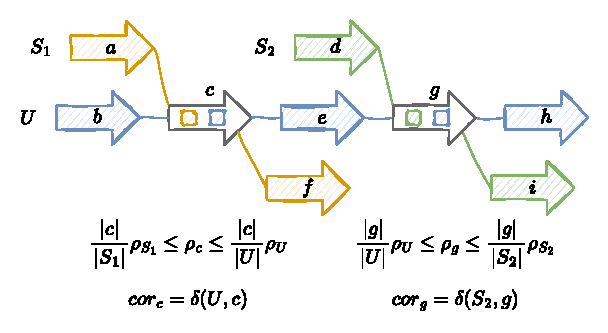
\includegraphics[width=0.6\linewidth]{pbf_iterbin/fine_tune/img/constraints-correct_plasmidness_example.pdf}
  \figurecaption{Differential correction of share fragment plasmidness.}{%
    Let assume the flow passes through all the link-arcs defining contigs \(U\), \(S_1\) and \(S_2\) (or their reverse).
    Because of the inequalities between the plasmidness, the objective function is corrected by \(\dplm{U}{c}\) for the share \(c\), and by \(\dplm{S_2}{g}\) for the share \(g\).
  }\label{fig:correct_share_plasmidness}
\end{figure}

\begin{todobox}
  Adpat best bonus GC prob score for plasmidness
\end{todobox}


% 
\usepackage{xcolor}

\AtBeginDocument{\colorlet{defaultcolor}{.}}

% Grey
\definecolor{drawio_grey}{HTML}{666666}
\definecolor{drawio_greyfill}{HTML}{F5F5F5}

% Blue
\definecolor{drawio_blue}{HTML}{6c8ebf} % 108 143 191
\definecolor{drawio_bluefill}{HTML}{dae8fc} % 218 232 252

\definecolor{drawio_darkblue}{HTML}{567299}
\definecolor{drawio_darkbluefill}{HTML}{aebaca}

% Turquoise
\definecolor{drawio_turquoise}{HTML}{64ABB3}
\definecolor{drawio_turquoisefill}{HTML}{D3E4E8}

% Green
\definecolor{drawio_green}{HTML}{82b366}
\definecolor{drawio_greenfill}{HTML}{d5e8d4}

\definecolor{drawio_darkgreen}{HTML}{33A02C}
\definecolor{drawio_darkgreenfill}{HTML}{B2DF8A}

% Orange
\definecolor{drawio_orange}{HTML}{d79b00}
\definecolor{drawio_orangefill}{HTML}{ffe6cc}

\definecolor{drawio_darkorange}{HTML}{FF7F00}
\definecolor{drawio_darkorangefill}{HTML}{FDBF6F}

% Yellow
\definecolor{drawio_yellow}{HTML}{d6b656}
\definecolor{drawio_yellowfill}{HTML}{fff2cc}

% Red
\definecolor{drawio_red}{HTML}{b85450}
\definecolor{drawio_redfill}{HTML}{f8cecc}

\definecolor{drawio_darkred}{HTML}{E31A1C}
\definecolor{drawio_darkredfill}{HTML}{FB9A99}

% Purple
\definecolor{drawio_purple}{HTML}{9673a6}
\definecolor{drawio_purplefill}{HTML}{e1d5e7}

\newcommand{\accentcolor}{drawio_yellow}

\hypersetup{linkcolor=drawio_red}
\hypersetup{citecolor=drawio_green}
% \hypersetup{linkcolor=defaultcolor}
% \hypersetup{citecolor=defaultcolor}
\setlist[description]{font=\sffamily\bfseries}
% ============================================================================ %
%                                 CUSTOM SPACES                                %
% ============================================================================ %
\let\oldforall\forall%
\renewcommand{\forall}{\oldforall{}\, }

\let\oldexist\exists%
\renewcommand{\exists}{\oldexist{}\: }

\newcommand{\existsu}{\oldexist! \: }

% ============================================================================ %
%                                   EQUATION                                   %
% ============================================================================ %
\usepackage{mathtools}

\usepackage{zref-clever}

%
% Constraints
%
\newcounter{constraint}

\zcRefTypeSetup{constraint}{
  name-sg = constraint,
  name-pl = constraints,
  Name-sg = Constraint,
  Name-pl = Constraints,
  refbounds={,C,,},
}
\newtagform{Const}{(C}{)}

\makeatletter
\NewDocumentEnvironment{Constraint}{}{%
  \usetagform{Const}%
  \zcsetup{reftype=constraint}%
  \let\c@equation\c@constraint\def\theequation{\theconstraint}%
}{}
\makeatother

%
% Objective functions
%
\newcounter{objective}

\zcRefTypeSetup{objective}{
  name-sg = objective,
  name-pl = objectives,
  Name-sg = Objective,
  Name-pl = Objectives,
  refbounds={,O,,},
}

\newtagform{Obj}{(O}{)}

\makeatletter
\NewDocumentEnvironment{Objective}{}{%
  \usetagform{Obj}%
  \zcsetup{reftype=objective}%
  \let\c@equation\c@objective\def\theequation{\theobjective}%
}{}
\makeatother
% ============================================================================ %
%                                    CAPTION                                   %
% ============================================================================ %
\usepackage{caption}
\usepackage{subcaption}
% ---------------------------------------------------------------------------- %
%                                      All                                     %
% ---------------------------------------------------------------------------- %
\captionsetup{labelfont=bf,font=sf}

% ---------------------------------------------------------------------------- %
%                                     Main                                     %
% ---------------------------------------------------------------------------- %
\captionsetup[figure]{%
  position=bottom,
  name={\textcolor{\accentcolor}{\(\blacksquare{}\)} Figure},
  labelsep=endash%
}
\captionsetup[table]{%
  position=top,
  name={\textcolor{\accentcolor}{\(\blacksquare{}\)} Table},
  labelsep=endash%
}
\captionsetup[longtable]{%
  position=top,
  name={\textcolor{\accentcolor}{\(\blacksquare{}\)} Table},
  labelsep=endash%
}
%
% Figure and table captions format
%
\newcommand{\figurecaption}[2]{%
  \caption[#1]{%
    \textbf{#1}%
    \ifstrempty{#2}
    {\ignorespaces}
    {\\ #2}%
  }%
}
\newcommand{\tablecaption}[2]{%
  \caption[#1]{%
    \textbf{#1}%
    \ifstrempty{#2}
    {\ignorespaces}
    {\\ #2}%
  }%
}
\newcommand{\longtablecaption}[2]{%
  \caption[#1]{%
    \textbf{#1}%
    \ifstrempty{#2}
    {\ignorespaces}
    {\\ #2}%
  }%
}
%
%   - captionof
%
\newcommand{\figurecaptionof}[2]{%
  \captionof{figure}[#1]{%
    \textbf{#1}%
    \ifstrempty{#2}
    {\ignorespaces}
    {\\ #2}%
  }%
}
% #XXX don't know why, but \tablecaption won't work and \tablecaptionof  must be use.
%   More surprisingly, \tablecaption must be kept in order to \tablecaptionof works!
%   But it works for \longtablecaption (according to caption pkg, captionof does not work for longtable)
\newcommand{\tablecaptionof}[2]{%
  \captionof{table}[#1]{%
    \textbf{#1}%
    \ifstrempty{#2}
    {\ignorespaces}
    {\\ #2}%
  }%
}

% ---------------------------------------------------------------------------- %
%                                      Sub                                     %
% ---------------------------------------------------------------------------- %
\captionsetup[subfigure]{position=bottom, labelfont=bf}
\captionsetup[subtable]{position=top, labelfont=bf}
%
% To use to describe subfigure in caption
%
\DeclareCaptionLabelFormat{parenth}{(#2)}
\captionsetup{subrefformat=parenth}
\newcommand{\Subref}[1]{\textbf{\subref{#1}}}

% ============================================================================ %
%                                 TABLE HEADERS                                %
% ============================================================================ %
\newcommand{\tabhtxt}[1]{\textbf{\sffamily{#1}}}
\newcommand{\tabhmath}[1]{\ensuremath{\mathsf{#1}}}

% ============================================================================ %
%                                    STYLES                                    %
% ============================================================================ %
\usepackage{tcolorbox}
\usepackage{booktabs} % for rule properties

\tcbuselibrary{skins}
\tcbuselibrary{breakable}

\tcbset{
  booktabsindent/.style={
    empty,
    breakable,
    % Title ---
    before title={\(\blacktriangleright{}\)},
    coltitle=black,
    fonttitle=\sffamily\bfseries,
    % Spaces ---
    left=0pt,
    toptitle=\aboverulesep,
    bottomtitle=\belowrulesep,
    % Inner text ---
    parbox=false,
    fontupper=\sffamily,
    % Border line ---
    titlerule style={black!75!white},
    titlerule=\lightrulewidth,
    leftrule=0pt, rightrule=0pt,% they hide titlerule
    borderline horizontal={\heavyrulewidth}{0pt}{black!75!white},
  },
  booktabsnoindent/.style={
    empty,
    boxsep=0pt,
    coltitle=black, fonttitle=\sffamily\bfseries,
    left=0mm, right=0mm,
    leftrule=0pt, rightrule=0pt,
    toptitle=\aboverulesep+1mm,
    bottomtitle=\belowrulesep+1mm,
    borderline horizontal={\heavyrulewidth}{0pt}{black!75!white},
    titlerule style={black!75!white},
    titlerule=\lightrulewidth%
  },
  roundbox/.style={
    enhanced jigsaw,
    boxsep=0pt,
    colframe=black!75!white,
    colback=white,
    boxrule=\heavyrulewidth,
    colbacktitle=white,
    sharp corners, rounded corners=all,
    coltitle=black, fonttitle=\sffamily\bfseries,
    toptitle=\aboverulesep+1mm,
    bottomtitle=\belowrulesep+1mm,
    titlerule style={black!75!white},
    titlerule=\lightrulewidth%
  },
  boxtitle/.style={
    enhanced,
    attach boxed title to top center={yshift*=-\tcboxedtitleheight/2},
    boxed title style={colback=white, boxrule=\lightrulewidth},
    boxsep=0pt,
    colframe=black!75!white,
    colback=white,
    boxrule=\heavyrulewidth,
    colbacktitle=white,
    sharp corners, rounded corners=all,
    coltitle=black, fonttitle=\sffamily\bfseries,
    toptitle=\aboverulesep+1mm,
    bottomtitle=\belowrulesep+1mm,
    titlerule style={black!75!white}
  },
  boxtitlenoindent/.style={
    empty,
    attach boxed title to top text left={yshift*=-\tcboxedtitleheight/2},
    boxed title style={
      skin=enhanced, colback=white, boxrule=\lightrulewidth,
      sharp corners, rounded corners=all, colframe=black!75!white
    },
    boxsep=0pt,
    coltitle=black, fonttitle=\sffamily\bfseries,
    left=0mm, right=0mm,
    leftrule=0pt, rightrule=0pt,
    toptitle=\aboverulesep+1mm,
    bottomtitle=\belowrulesep+1mm,
    borderline horizontal={\heavyrulewidth}{0pt}{black!75!white},
    titlerule=\lightrulewidth%
  },
  % leftlineindent/.style={
  %   empty,
  %   breakable,
  %   % Title ---
  %   minipage boxed title,
  %   attach boxed title to top left,
  %   boxed title style={
  %     empty,
  %     left*=0pt,
  %   },
  %   coltitle=black,
  %   fonttitle=\sffamily\bfseries,
  %   before title={\(\blacktriangleright{}\)},
  %   % Inner text ---
  %   parbox=false,
  %   fontupper=\sffamily,
  %   % Border line ---
  %   borderline west={\heavyrulewidth}{4pt}{black!75!white},
  % },
  leftlineindent/.style={
    empty,
    breakable,
    % Title ---
    % minipage boxed title,
    % attach boxed title to top left,
    % boxed title style={
    %   empty,
    %   left*=0pt,
    % },
    coltitle=black,
    fonttitle=\sffamily\bfseries,
    before title={\(\blacksquare{}\)~},
    % before title={\(\blacktriangleright{}\)},
    % Inner text ---
    parbox=false,
    fontupper=\sffamily,
    % Border line ---
    % borderline west={\heavyrulewidth}{4pt}{black!75!white},
    borderline west={\heavyrulewidth}{0pt}{black!75!white},
  },
  proofempty/.style={
    empty,
    breakable,
    % Title ---
    attach boxed title to top left,
    boxed title style={
      empty,
      left*=0pt,
    },
    coltitle=black,
    fonttitle=\sffamily,
    title=\(\rhd{}\) Proof,
    % Inner text ---
    parbox=false,
    fontupper=\itshape,
    % End of box ---
    after upper={\par\hfill \(\lhd{}\)},
  },
}

\usepackage{biblatex}
\stdpunctuation% else biblatex-ieee will print the comma before the closing french quote
\AtEveryCitekey{%
  \clearfield{url}%
  \clearfield{urlyear}%
}

% ============================================================================ %
%                                   PACKAGES                                   %
% ============================================================================ %
\usepackage[indLines=false]{algpseudocodex}

% ============================================================================ %
%                            CUSTOM SIMPLE STATEMENT                           %
% ============================================================================ %
\newcommand{\Assert}{\textbf{\sffamily{assert}} }

% ============================================================================ %
%                                     LOOP                                     %
% ============================================================================ %
% ---------------------------------------------------------------------------- %
%                                    FromTo                                    %
% ---------------------------------------------------------------------------- %
\algnewcommand\algorithmicfromto{\textbf{for}}%

\makeatletter
\algdef{SE}[FROMTO]{FromTo}{EndFromTo}[3]{\algpx@startIndent\algpx@startCodeCommand\algorithmicfromto\ #1\ \textbf{from}\ #2\ \textbf{to}\ #3\ \algorithmicdo}{\algpx@endIndent\algpx@startCodeCommand\algorithmicend\ \algorithmicfromto}%

\ifbool{algpx@noEnd}{%
  \algtext*{EndFromTo}%
  %
  % end indent line after (not before), to get correct y position for multiline text in last command
  \apptocmd{\EndFromTo}{\algpx@endIndent}{}{}%
}{}%

\pretocmd{\FromTo}{\algpx@endCodeCommand}{}{}

% for end commands that may not be printed, tell endCodeCommand whether we are using noEnd
\ifbool{algpx@noEnd}{%
  \pretocmd{\EndFromTo}{\algpx@endCodeCommand[1]}{}{}%
}{%
  \pretocmd{\EndFromTo}{\algpx@endCodeCommand[0]}{}{}%
}%
\makeatother


% ============================================================================ %
%                                  DELIMITERS                                  %
% ============================================================================ %
% ---------------------------------------------------------------------------- %
%                                  Parenthesis                                 %
% ---------------------------------------------------------------------------- %
%
% Usage: \parenth*{...} or \parenth[\big]{...}
%
\DeclarePairedDelimiterX{\parenth}[1]{(}{)}{#1}  % chktex 9

% ---------------------------------------------------------------------------- %
%                                      Set                                     %
% ---------------------------------------------------------------------------- %
%
% Usage: \Set*{... \given ...} or \Set[\big]{...}
%
\providecommand\given{} % just to make sure it exists
\newcommand\SetSymbol[1][]{%
  \nonscript{}\:#1\vert%
  \allowbreak%
  \nonscript{}\:
  \mathopen{}
}
\DeclarePairedDelimiterX{\Set}[1]{\{}{\}}{%
  \renewcommand\given{\SetSymbol[\delimsize]}
  #1
}

% Require:
% \input{custom/format/color}

\usepackage{fontawesome5}
\usepackage{booktabs}
\usepackage{tcolorbox}

\tcbuselibrary{skins}
\tcbuselibrary{breakable}

%
% USAGE:
%
%   \boxfactory{boxname}{title}{color}
\newcommand{\boxfactory}[3]{
  \newtcolorbox{#1}{
    empty,
    breakable,
    % Title ---
    boxed title style={
      empty,
      left*=0pt,
    },
    title=#2,
    coltitle=#3,
    fonttitle=\sffamily\bfseries,
    % Inner text ---
    parbox=false,
    coltext=drawio_grey,
    fontupper=\sffamily,
    % Border line ---
    borderline west={2\heavyrulewidth}{0pt}{#3},
  }
}

\boxfactory{notebox}{\faIcon{pencil-alt} Note}{drawio_grey}
\boxfactory{infobox}{\faIcon{info-circle} Info}{drawio_darkblue}
\boxfactory{warningbox}{\faIcon{exclamation-triangle} Warning}{drawio_orange}
\boxfactory{questionbox}{\faIcon{question-circle} Question}{drawio_purple}
\boxfactory{ideabox}{\faIcon{lightbulb} Idea}{drawio_yellow}
\boxfactory{errorbox}{\faIcon{times-circle} Error}{drawio_red}
\boxfactory{todobox}{\faIcon{check-circle} To-do}{drawio_darkgreen}
\boxfactory{missingproofbox}{\faIcon{stop} Missing proof}{drawio_turquoise}
\boxfactory{refactorbox}{\faIcon{recycle} Refactor}{drawio_darkgreen}
\boxfactory{fixmebox}{\faIcon{wrench} Fix-me}{drawio_red}
\boxfactory{newfeatbox}{\faIcon{star} New feature}{drawio_yellow}
\boxfactory{cleanupbox}{\faIcon{broom} Clean-up}{drawio_yellow}
% ============================================================================ %
%                                    SYMBOLS                                   %
% ============================================================================ %
\newcommand{\tobij}{%
  \hookrightarrow\mathrel{\mspace{-15mu}}\rightarrow%
}
\newcommand{\tosur}{%
  \rightarrow\mathrel{\mspace{-15mu}}\rightarrow%
}
\newcommand{\toinj}{%
  \hookrightarrow%
}

% ============================================================================ %
%                                     SETS                                     %
% ============================================================================ %
\newcommand{\Reals}{\ensuremath{\mathbb{R}}}
% ============================================================================ %
%                                 NEW THEOREMS                                 %
% ============================================================================ %
% Require
\usepackage{tcolorbox}
\tcbuselibrary{theorems}
% Need: \input{custom/format/tcolorbox}
\usepackage{zref-clever}
% ---------------------------------------------------------------------------- %
%                                   Algorithm                                  %
% ---------------------------------------------------------------------------- %
\newtcbtheorem[
  list inside=algorithm,
]{tcbalgo}{Algorithm}{booktabsindent,before upper*=\sf,label type=algo}{algo}
\zcRefTypeSetup{algo}{
  Name-sg=Algorithm,
  name-sg=algorithm,
  Name-pl=Algorithms,
  name-pl=algorithms,
}

% ---------------------------------------------------------------------------- %
%                                 Theorem Like                                 %
% ---------------------------------------------------------------------------- %
\newtcbtheorem[
  number within=section,
  list inside=definition
]{definition}{Definition}{leftlineindent,label type=definition}{definition}
\zcRefTypeSetup{definition}{
  Name-sg=Definition,
  name-sg=definition,
  Name-pl=Definitions,
  name-pl=definitions,
}
\newtcbtheorem[
  number within=section,
  list inside=property
]{property}{Property}{leftlineindent,label type=property}{property}
\zcRefTypeSetup{property}{
  Name-sg=Property,
  name-sg=property,
  Name-pl=Properties,
  name-pl=properties,
}

\newtcbtheorem[
  number within=section,
  list inside=axiom
]{axiom}{Axiom}{leftlineindent,label type=axiom}{axiom}
\zcRefTypeSetup{axiom}{
  Name-sg=Axiom,
  name-sg=axiom,
  Name-pl=Axioms,
  name-pl=axioms,
}

\newtcbtheorem[
  number within=section,
  list inside=postulate
]{postulate}{Postulate}{leftlineindent,label type=postulate}{postulate}
\zcRefTypeSetup{postulate}{
  Name-sg=Postulate,
  name-sg=postulate,
  Name-pl=Postulates,
  name-pl=postulates,
}

\newtcbtheorem[
  number within=section,
  list inside=theorem
]{theorem}{Theorem}{leftlineindent,label type=theorem}{theorem}
\zcRefTypeSetup{theorem}{
  Name-sg=Theorem,
  name-sg=theorem,
  Name-pl=Theorems,
  name-pl=theorems,
}

\newtcbtheorem[
  number within=section,
  list inside=proposition
]{proposition}{Proposition}{leftlineindent,label type=proposition}{proposition}
\zcRefTypeSetup{proposition}{
  Name-sg=Proposition,
  name-sg=proposition,
  Name-pl=Proposition,
  name-pl=propositions,
}

\newtcbtheorem[
  number within=section,
  list inside=lemma
]{lemma}{Lemma}{leftlineindent,label type=lemma}{lemma}
\zcRefTypeSetup{lemma}{
  Name-sg=Lemma,
  name-sg=lemma,
  Name-pl=Lemmas,
  name-pl=lemmas,
}

% ---------------------------------------------------------------------------- %
%                                     Proof                                    %
% ---------------------------------------------------------------------------- %
\renewenvironment{proof}{
\begin{tcolorbox}[proofempty]}{
\end{tcolorbox}}

% ============================================================================ %
%                                   PACKAGES                                   %
% ============================================================================ %
% \input{custom/format/color}
\usepackage{etoolbox}
\usepackage{calc}
\usepackage{soul}

% ============================================================================ %
%                                 TODO BUILDER                                 %
% ============================================================================ %
%
% USAGE:
%
%   \todobuilder{\todoname}{todocolor_border}{todocolor_fill}
%
%   \todoname{toto text} % in the text
%   \todoname[inline]{toto text} % in full line width
%
% NOTE:
%
%   If the command breaks, try to \protect any non-text object (e.g. commands)
%   As an example:
%   \todotosay{blabla~\protect\cite{bib_entry}}
%
\newcommand{\todobuilder}[3]{
  \newcommand{#1}[2][]{%
    \expandafter\ifstrequal\expandafter{##1}{inline}{%
      \par\noindent
      {\sffamily{\bfseries \sethlcolor{#2}\hl{[#3] }}{\sethlcolor{#2}\hl{##2}}}
      \par
    }{%
      {\sffamily{\sethlcolor{#2}\hl{##2}}}%
    }%
  }
}

% ============================================================================ %
%                                 NEW COMMANDS                                 %
% ============================================================================ %
% ---------------------------------------------------------------------------- %
%                                    Remark                                    %
% ---------------------------------------------------------------------------- %
\todobuilder{\todoremark}{drawio_orangefill}{REMARK}

% ---------------------------------------------------------------------------- %
%                                     Error                                    %
% ---------------------------------------------------------------------------- %
\todobuilder{\todoerror}{drawio_redfill}{ERROR}

% ---------------------------------------------------------------------------- %
%                                     Proof                                    %
% ---------------------------------------------------------------------------- %
\todobuilder{\todoproof}{drawio_purplefill}{TO PROOF}

% ---------------------------------------------------------------------------- %
%                                    To Say                                    %
% ---------------------------------------------------------------------------- %
\todobuilder{\todotosay}{drawio_greenfill}{TO SAY}

% ---------------------------------------------------------------------------- %
%                                  To Arrange                                  %
% ---------------------------------------------------------------------------- %
\todobuilder{\todoarrange}{drawio_bluefill}{TO REFACTOR}


